\documentclass[12pt,italian]{article}
\usepackage[margin=1in]{geometry}
\setlength{\parskip}{5pt}
\usepackage[utf8]{inputenc} 
\usepackage[italian]{babel}
\usepackage{hyperref}
\usepackage{float}
\usepackage{times}
\usepackage{titling}
\usepackage{graphicx}
\usepackage{blindtext}
\usepackage{csquotes}
\usepackage{filecontents}
\usepackage{titlesec}
\newcommand{\sectionbreak}{\clearpage}
\usepackage[
backend=biber,
]{biblatex}
\addbibresource{bibliography.bib}

\title{PPS18  --- Spark-external-internal-analysis}
\author{Chiara Forresi, matr: 880050, email: {\url{chiara.forresi@studio.unibo.it}}}
\date{\today}

\begin{document}

\begin{titlingpage}
	\maketitle
	\begin{abstract}
		Spark è un famoso framework Scala per big-data e cluster computing. In questo progetto si studieranno aspetti linguistici di questo framework, e la sua organizzazione interna -- l'obiettivo è porre le basi per futuri framework per computazione distribuita che si ispirino a Spark.
	\end{abstract}
\end{titlingpage}
\nocite{*}
\tableofcontents
\newpage

\section{Cos'è Spark?}
Spark non è solo un motore di elaborazione di big data, può essere considerato un ``ecosistema" che offre svariate possibilità.
Si tratta di una completa alternativa al `map-reduce' di Hadoop \footnote{\url{https://hadoop.apache.org/docs/r1.2.1/mapred\_tutorial.html}}, con molti vantaggi in termini di performance. 
\par Alla base dell'ecosistema di Spark vi è \textbf{SparkCore}, il quale, a sua volta, è diviso in due parti:
\begin{itemize}
	\item \textbf{Computer Engine}: fornisce funzioni basilari come gestione della memoria, scheduling dei task, recupero guasti, interagisce con il Cluster Manager (che non viene fornito da Spark).
	\item \textbf{Spark Core} APIS che consiste in due API:
	\begin{itemize}
		\item strutturate: DataFrame e Dataset, ottimizzate per lavorare con dati strutturati
		\item non strutturate: RDDs, variabili Accumulators e Broadcast
	\end{itemize}
\end{itemize}
Sopra a \textit{SparkCore} troviamo principalemente, come mostrato in Figura \ref{fig:SparkModules}, i seguenti moduli:
\begin{itemize}
	\item \textbf{Spark SQL}
	\item  \textbf{Spark Streaming}
	\item \textbf{MLlib}
	\item \textbf{GraphX}
\end{itemize}
Essi offrono API, DLS e algoritmi in più linguaggi e dipendono direttamente dalla base, ovvero SparkCore. Verranno approfonditi più avanti.
\begin{figure}[H]
	\centering 
	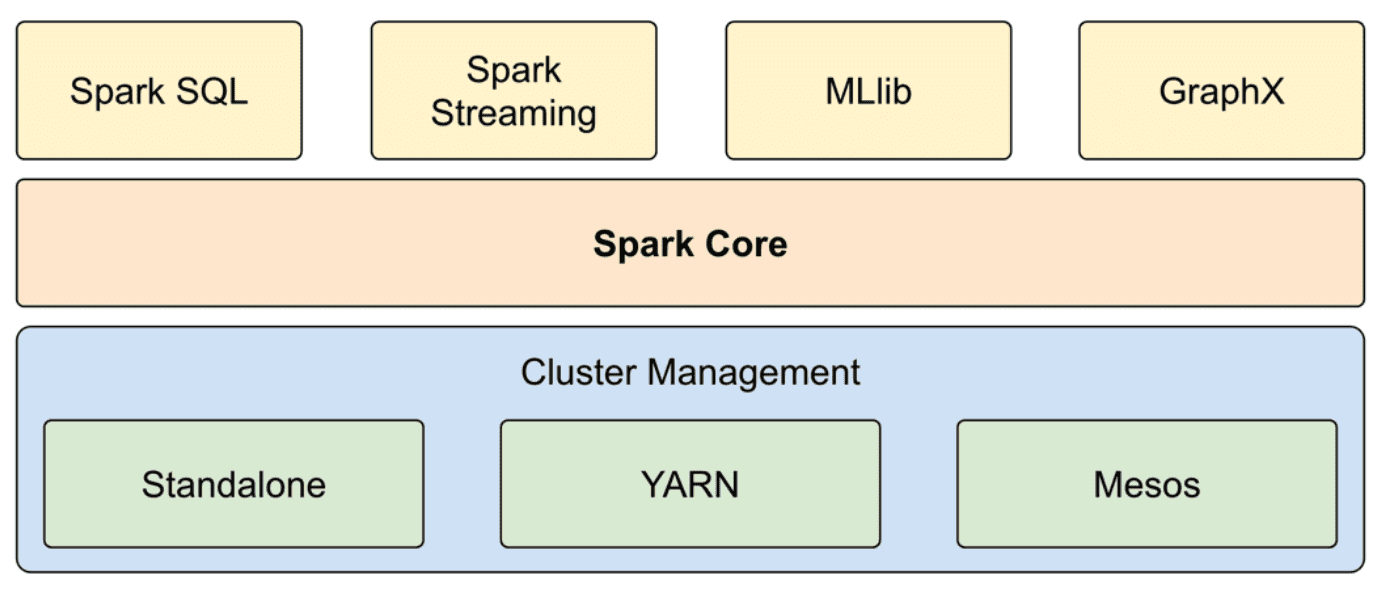
\includegraphics[width=0.8\linewidth]{img/sparkModules.png}
	\caption{Archiettura di Spark. Immagine tratta da \url{https://docs.incorta.com/}}
	\label{fig:SparkModules}
\end{figure}
\par Vista la varietà di funzionalità che Spark offre, in questo progetto ci si focalizzerà maggiormente sulle funzionalità di SparkCore e sulle modalità di gestione di Streaming di dati. In entrambi i casi l'analisi verrà svolta si da un punto di vista estereriore di quello che offre il framework che quello interiore, andando a sviscerare le caretteristiche e i punti peculiari (positivi o negativi) che emergono dall'analisi. 
\newline
Si sottolinea che in questo progetto è stata utilizzata l'ultima versione disponibile di Spark, ovvero la \textbf{2.4.4}. Per cui per maggiori dettagli si rimanda al sito di Spark \cite{spark}.
\subsection{Perchè Spark è così importante?}
L'importanza di Spark è data soprattutto dal fatto che in un'unico framework vengono create interesioni di vario genere che fanno si che esso sia una piattaforma a tutto tondo. Questi punti sintetizzano i motivi principali dell'importanza di Spark:
\begin{itemize}
	\item Astrae la programmazione parallela, non sembra di lavorare su un cluster di computer.
	Nello scenario migliore sembrerà di lavorare con un database (SQL), nel peggiore di lavorare su Collections.
	\item Piattaforma unificata, tutto in un singolo framework.
	\item Facile da usare, leggere e capire.
\end{itemize}
\subsection{Un primo approccio a Spark}
Per prendere confidenzialità con Spark, così come abbiamo fatto con Scala, può essere utile utilizzare la REPL (anche nota come \textbf{spark-shell}). 
Utilizzarla con Spark è molto semplice:
\begin{itemize}
	\item basta andare nell'url \url{https://spark.apache.org/downloads.html} e scaricare l'ultima versione di Spark compresa di Hadoop;
	\item decomprimere la cartella e posizionarsi all'interno di essa da terminale;
	\item a questo punto lanciando il comando \texttt{./bin/spark-shell} partirà la shell.
\end{itemize}
Si può anche memorizzare questo percorso nel path di sistema e accedervi da qualsiasi parte del file system. Aggiungendo a ~/.bashrc:
\begin{itemize}
	\item \texttt{export SPARK\_HOME="percorso della cartella decompressa"} 
	\item \texttt{export PATH=$PATH:$SPARK\_HOME/bin:\$SPARK\_HOME/sbin}
\end{itemize}

Seguendo il tutoria \cite{localexample} è possibile mettere le mani in pasta in locale su un dataset e esplorare le potenzialità di Spark (in particolare Spark SQL) e, soprattutto, del DLS che esso fornisce.
\section{Internals}
\subsection{Architettura}
É possibile lanciare Spark essenzialmente in \textbf{due modalità}:
\begin{enumerate}
	\item \textbf{interattiva}
	\item \textbf{submit di un job} (in caso di produzione). 
\end{enumerate}
Queste modalità ci aprono al concetto di \textit{master-worker} (PCD) che nel ``dialetto di Spark" è noto come \textbf{``driver-executor"}.
Essenzialmente posso usare Spark con o senza un vero cluster:
\begin{itemize}
	\item \textbf{local mode}: uso in fase esplorativa per iniziare ad usare spark senza un effettivo cluster.
	\item \textbf{con cluster}
	\begin{itemize}
		\item \textbf{client mode}: il driver è nel client, per cui è preferibile usarla in fase di debug;
		\item \textbf{cluster mode}: il driver è nel cluster, la uso in produzione.
	\end{itemize}
\end{itemize}
Quando eseguo Spark lo stato dei processi è visibile in una pagina web che viene linkata nel esecuzione del progesso (la \textbf{Spark UI}), in essa è possibile visualizzare come viene effettivamente distribuito il lavoro, lo stato del lavoro e i DAG. %TODO

\textit{Chi controlla il cluster? Come Spark ottiene le risorse per driver e executor?}
Il \textit{cluster manager}, il quale non viene offerto da Apache Spark. Tra i più noti abbiamo:
\begin{itemize}
	\item\textbf{Apache YARN\footnote{\url{http://hadoop.apache.org/docs/stable/hadoop-yarn/hadoop-yarn-site/YARN.html}}}: il gestore delle risorse in Hadoop 2.
	\item\textbf{Apache Mesos\footnote{\url{http://mesos.apache.org}}}: generale che può anche eseguire Hadoop MapReduce e le applicazioni di servizio.
	\item\textbf{Kubernetes\footnote{\url{https://kubernetes.io}}}: un sistema open source per automatizzare la distribuzione, il ridimensionamento e la gestione di applicazioni containerizzate. Non ancora adatto per fasi di produzione.
	\item\textbf{Standalone\footnote{\url{https://spark.apache.org/docs/latest/spark-standalone.html}}}: semplice, facile e veloce. Incluso in Spark, semplifica la configurazione di un cluster. Non ancora adatto per fasi di produzione. 
\end{itemize}


\subsection{RDDs  e tasks}
\subsubsection{Resilient Distributed Datasets (RDDs)}
Spark ruota attorno al concetto di RDD, ovvero una collection fault-tollerant che può essere processata in parallelo. Ci sono due modi per creare un RDD: parellelizzando una collezione esistente nel tuo driver program o facendo riferimento a un archivio di dati esterno (come filesystem condivisi, HDFS, Hbase o qualsiasi input che ha dati in formato Hadoop).

\subsubsection{RDDs e conseguenze}
Poichè Dataset e DataFrame (API di dati strutturati) ereditano da RDDs (non strutturati), capendo questi ultimi possiamo capire come effettivamente viene distribuito il lavoro tra gli executors.

Quando viene letto un file è possibile specificare il numero di \textbf{partizioni di un RDD} che (guarda caso) coincide con il corrispondente \textbf{numero di task}.
Ovviamente, numero executors e di task sono effettivamente correlati e quindi bisogna specificare il numero di conseguenza.

Si lavora in \textbf{stage}, uno stage rappresenta un periodo (una o più funzione chiamata sui dati) in cui non è necessario uno shuffle, ovvero non è necessario spostare i dati tra le partizioni. Se i dati devono muoversi (es. reduceByKey) bisogna ripartizionare i dati (\textit{shuffle \& sort}).
Con `collect` si ritorna dagli executor al driver.

%TODO Nota interessante, in Scala, DataFrame è così definito ``type DataFrame = Dataset[Row]" \footnote{\url{https://spark.apache.org/docs/2.4.4/api/scala/index.html}}, ciò significa che su un DataFrame posso chiamare tutti i metodi del Dataset.

\subsection{Execution Model} %TODO
\begin{itemize}
	\item Crea DAG di RDDs per rappresentare la computazione;
	\item Crea piano di esecuzione logico del DAG;
	\item pipeline il più possibile %TODO
	\item divide in \textbf{stages}
	\item Schedula e esegue i tasks:
	\item divide ogni stage in task
	\item task = dati + computazione
	\item esegue tutti i task di uno stage prima di andare avanti
\end{itemize}

\subsection{Di più sullo shuffle}
Note importanti sullo shuffle sono:
\begin{enumerate}
	\item è pull based e non push based;
	\item scrive file intermedi nei dischi
\end{enumerate}
Bisognate tenere d'occhio il \textbf{numero di partizioni} perchè possono fondamentalmente esserci due situazioni.
\begin{enumerate}
	\item numero troppo \textbf{basso}:
	\begin{itemize}
		\item poca concorrenza
		\item più suscettibile a \textit{``data skew"} (spostamento di dati)
		\item maggiore uso della memoria in operazioni che richiedono Shuffle (groupBy, sortByKey, reduceByKey, etc.)
	\end{itemize}
	\item numero troppo \textbf{alto}: problemi opposti, dati troppo sparsi e non viene sfruttato il partizionamento.
\end{enumerate}
Un numero appropiato di solito è tra 100 e 10000.
Bisogna fissare questo numero nell'intervallo compreso tra:
\begin{itemize}
	\item \textbf{lower bound}:  almeno circa il doppio del numero di core di un cluster;
	\item \textbf{upper bound}: essere sicuri che un task venga eseguito in almeno 100ms.
\end{itemize}

%TODO (da vedere https://databricks.com/session/a-deeper-understanding-of-spark-internals da min. 22)

\section{Moduli di Spark}
\subsection{Iniziare a lavorarare con Spark e gli RDDs}
Per iniziare a usare Spark bisogna comprendere il concetto principale di \textit{SparkContext}.
Per ciascuna JVM ci può essere al più una \textit{SparkContext}, si tratta del il punto di ingresso principale per la funzionalità Spark. Uno SparkContext rappresenta la connessione a un cluster Spark e può essere utilizzato per creare RDD, accumulatori e trasmettere variabili su quel cluster. 

A uno SparkContext bisogna fornire una configurazione che nel caso generale corrisponde a SparkConf. Nel caso in cui si usano Dataset e DataFrame API, la \textit{SparkSession} facilità la configurazione con un builder dal quale poi si ottiene un'instanza di SparkContext. 
%TODO example???
\par Ci sono due operazioni fondamentali che vengono fatte sui dati, che rispecchiano essenzialemente il principio \textit{map-reduce}:
\begin{itemize}
	\item \textbf{transformations}: ovvero operazioni di map \textit{map}, sono lazy l'eventuale azione su di essa applicherà la trasformazione. Eventualmente è possibile rendere questi cambiamenti persistenti (con l'opportuno persist), altrimenti non lo sono.
	\item \textbf{actions}: ovvero operazioni di map \textit{reduce}.
\end{itemize}
La Figura \ref{fig:RDDs} mostra l'intero meccanismo di RDDs e trasformazioni e azioni.
\begin{figure}
	\centering 
	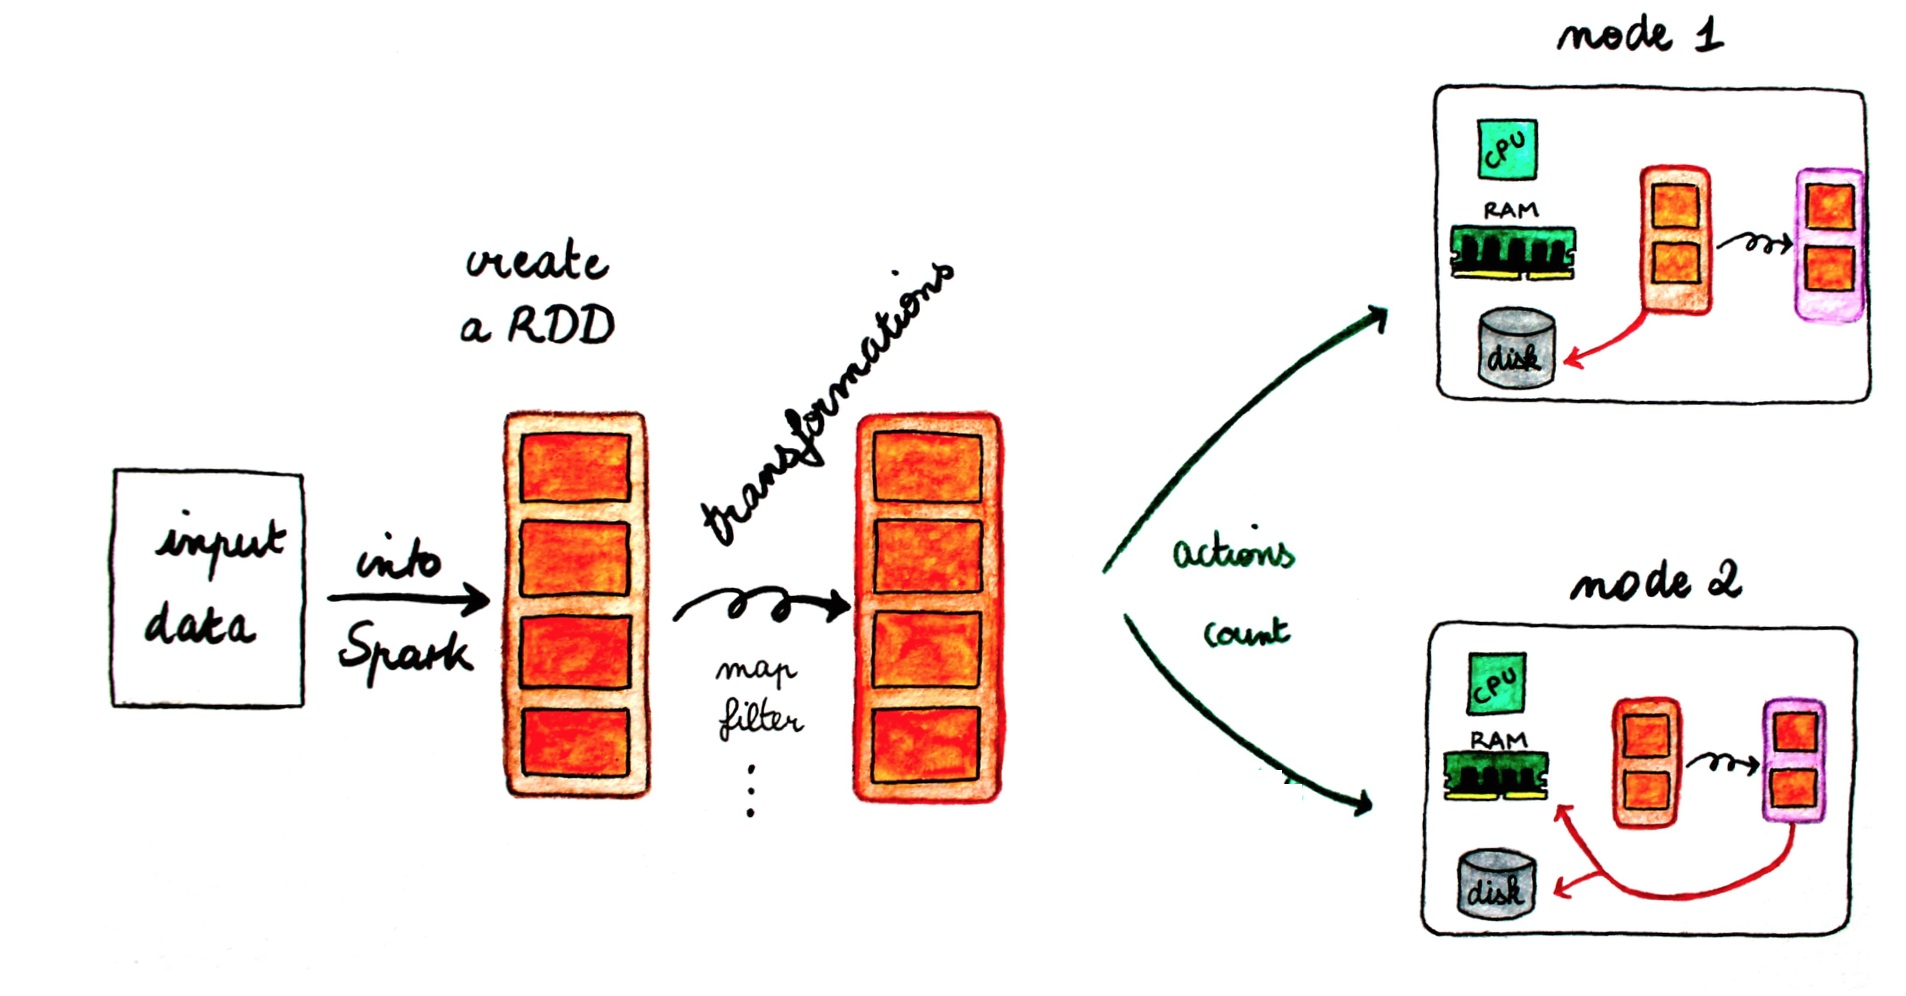
\includegraphics[width=1\linewidth]{img/rdds.png}
	\caption{RDDs e meccanismo di trasformations e actions.https://docs.incorta.com/ \url{http://sparkforbeginners.blogspot.com}}
	\label{fig:RDDs}
\end{figure}
\par Per passare funzioni a Spark nel sito viene mostrato come sfruttare map su un RDDs applicandoci una propria funzione che prende in input un dato dello stresso tipo di quello contenuto nel RDDs. Secondo me questo aspetto da un lato obbliga il programmatore ad appoggiarsi alle API fornite dal framework e quindi ottimizzate da Spark, dall'altro pone dei limiti nel come il programmatore vuole approcciarsi ai dati. Limite che viene abbastanza ridotto dalla potenza e dalla facilità di comprensione del DLS che Spark mette a disposizione.
\par Per quanto riguarda il \textbf{caching}, oltre a persistent, esistono modalità per specificare a quale memoria far riferimento e funziona anche su dati presenti in molti nodi.
\par Se andassi ad applicare \texttt{collect()} su una grande quantità di dati potrei incorrere in un \textit{``out of memory"}, per cui bisogna applicare concetti simili a quelli visti durante il corso di PPS. Ad esempio anzichè fare una stampa di tutti i dati, si vanno recuperare i primi N record con una \texttt{take(N)}.
\par Una delle cose più difficili di Spark è comprendere l'ambito e il ciclo di vita di variabili e metodi quando si esegue il codice in un cluster. Le operazioni RDD che modificano le variabili al di fuori del loro ambito di applicazione possono essere una fonte frequente di confusione. C'è sostanzialmente un problema di concorrenza e della \textit{closure} rispetto all'ambito di lavoro di un task che Spark risolve con l'inserimento di due concetti:
%TODO meglio??
\begin{enumerate}
	\item \textbf{broadcasts}:  consentono al programmatore di mantenere una variabile di sola lettura memorizzata nella cache su ogni macchina anziché inviarne una copia con le attività. Possono essere utilizzati, ad esempio, per fornire ad ogni nodo una copia di un set di dati di input di grandi dimensioni in modo efficiente. Spark tenta anche di distribuire variabili di trasmissione utilizzando algoritmi di trasmissione efficienti per ridurre i costi di comunicazione.
	\item \textbf{accumulators}: sono variabili che vengono “aggiunte” solo attraverso un'operazione associativa e commutativa e possono quindi essere supportate in modo efficiente in parallelo. Possono essere utilizzati per implementare contatori (come in MapReduce) o somme. Spark supporta nativamente accumulatori di tipi numerici e i programmatori possono aggiungere il supporto per nuovi tipi. Vale sempre il concetto lazy (vedi trasformazioni).
\end{enumerate}
\subsection{Machine Learning Library (MLlib)}
Questo modulo consiste in:
\begin{itemize}
	\item \textit{Algoritmi di Machine Learning}: come classificazione, regressione, clustering e filtering collaborativo.
	\item \textit{Featurization}: estrazione delle feature, transformazione, riduzione della dimensionalità e selezione.
	\item \textit{Pipelines}: tool per costruire, valutare e fare tuning di pipeline di ML.
	\item \textit{Persistenza}: salvare e eseguire algoritmi, modelli e pipeline.
	\item \textit{Utility}: algebra lineare, statistica, gestione dati, etc.
\end{itemize}
\subsection{Spark SQL}
Supporto a dati strutturati, fornisce maggiori ottimizzazioni rispetto a RDD. L'interazione con i dati è possibile in vari modi, tra cui SQL e Dataset API.
Nella computazione viene usato un unico engine di esecuzione, il programmatore può esprire le cose nel modo che ritiene più naturale. Uso di Hive, JDBC, etc. 
Non credo questo sia interessante sul lato PPS. %TODO
\subsubsection{Dataset API}
Operazioni con cui interrogare il Dataset. 
Un Dataset si può creare anche ``on the fly" da un file di testo o appartenere a determinati formati (es. Hadoop HDFS) o trasformando altri Dataset.
Nelle interrogazioni che lo richiedono vengono passate funzioni, per cui possono entrare in gioco aspetti di PPS. Questa parte verrà meglio sviscerata in seguito. %TODOs
\subsection{GraphX Programming}
Componente Spark per Grafi e calcolo graph-parallel.

Ad alto livello viene estratto il concetto di RDD introducendo l'estensione Graph, in Figura \ref{fig:GraphX} viene mostrata la costruzione del grafo a partire dai dati grezzi.
Ci sono varie operazioni a supporto di questo concetto, anche algoritmi e builder per l'analisi.
\begin{figure}[H]
	\centering 
	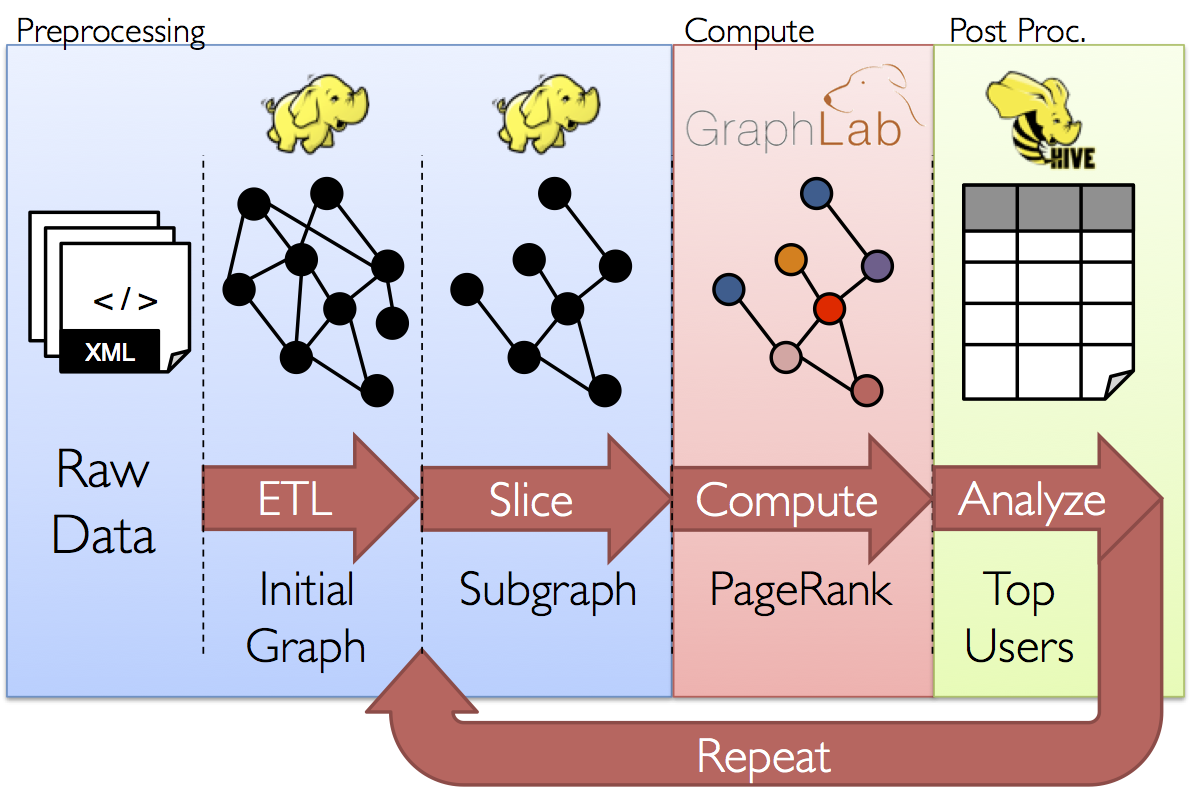
\includegraphics[width=0.8\linewidth]{img/graph_analytics_pipeline.png}
	\caption{Funzionamento di GraphX. Immagine tratta da \cite{spark}.}
	\label{fig:GraphX}
\end{figure}
Quindi userei questa estensione quando nella natura dei dati ci sono legami che vengono meglio rappresentati da un grafo,
prima di dare in pasto i dati a GraphX potrebbero servire minime operazioni per renderli "compatibili" con la visione a grafo.
Nella costruzione vengono richiesti:
\begin{itemize}
	\item RDD dei vertici;
	\item RDD degli edge;
	\item un vertice di default (pozzo).
\end{itemize}
\subsection{SparkR (R on Spark)}
SparkR è un pacchetto R che fornisce un frontend leggero per utilizzare Apache Spark da R. In Spark 2.4.4, SparkR fornisce un'implementazione di data frame distribuiti che supporta operazioni come selezione, filtro, aggregazione ecc. (simile a data frame R, dplyr) ma su set di dati di grandi dimensioni. SparkR supporta inoltre l'apprendimento automatico distribuito tramite MLlib.

\subsection{Moduli per lavorare con stream di dati}
\subsubsection{Spark Streaming}
Spark Streaming, come mostrato in Figura \ref{fig:SparkStreaming}, raccoglie dati provenienti da varie fonti (es. Kafka, Flume, Kinesis o TCP sockets, file) li processa usando algoritmi complessi espressi attravervo funzioni high-level come \textit{map}, \textit{reduce}, \textit{join} e \textit{window}, e inserisce il risultato in File Systems (HDFS), Databases o Dashboard da eventualemente elaborare con le funzioni di spark ML e Graph.

Internamente Spark Streaming divide lo stream in batch di dati che vengono processati dalla Spark Engine.

La lettura di uno streaming avviene tramite un \textbf{Receiver} ed eredita dall'astrazione \textbf{DStream}, si tratta di dati che provengono da varie fonti (es. Kafka, Flume, and Kinesis) o da operazione ad alto livello su altri DStream.
Un DStream può essere considerato come una sequenza di RDDs.

Fondamentale è la definizione di un \textit{Batch interval}, esso indica la durata secondo la quale uno Spark Streaming Job immagazzina dati e, per cui, in ogni intervallo ci sarà un DStream differente.
Questo concetto fa capire la forte nota di Spark Streaming nel lavorare in micro batch e non in real time, questo è essezialmente per maggiori performance \footnote{\url{https://sqlstream.com/5-reasons-why-spark-streamings-batch-processing-of-data-streams-is-not-stream-processing/}}. %TODO

Le \textbf{operazioni su un DStream}, molto simili a quelle su un RDD, funzioni proprie si possono applicare 
solo attraverso quelle fornite dall'API, questo è limitante rispetto allo Structured Stream.

Per usare Spark Streaming è necessario definire uno \textit{SparkStreamingContext}, per il quale bisogna definire uno \textit{StreamingContext} e un \textit{BatchInterval}.
Attraverso dei metodi preposti in questa struttura verranno consumati dati e creati di conseguenza i relativi DStream.

A volte non basta considerare un intervallo, ma è più opportuno considerare una finestra, per cui si passa da una transformazione Stateless in cui vengono scartati da batch precedenti) a una trasformazione Stateful. In particolare con lo \textbf{sliding windows} vengono aggregati DStream appartanenti a intervalli diversi.
Ci sono due ulteriori parametri, oltre al batch interval, da tarare:
\begin{itemize}
	\item \textbf{window size}: multiplo di batch interval, indica l'ampiezza temporale della finestra
	\item \textbf{slide window dimension}: indica quanta distanza temporale c'è tra una window e la successiva, anche esso è multiplo del batch interval e potenzialmente potrebbero esserci finestre sovrapposte.
\end{itemize}
\begin{figure}
	\centering 
	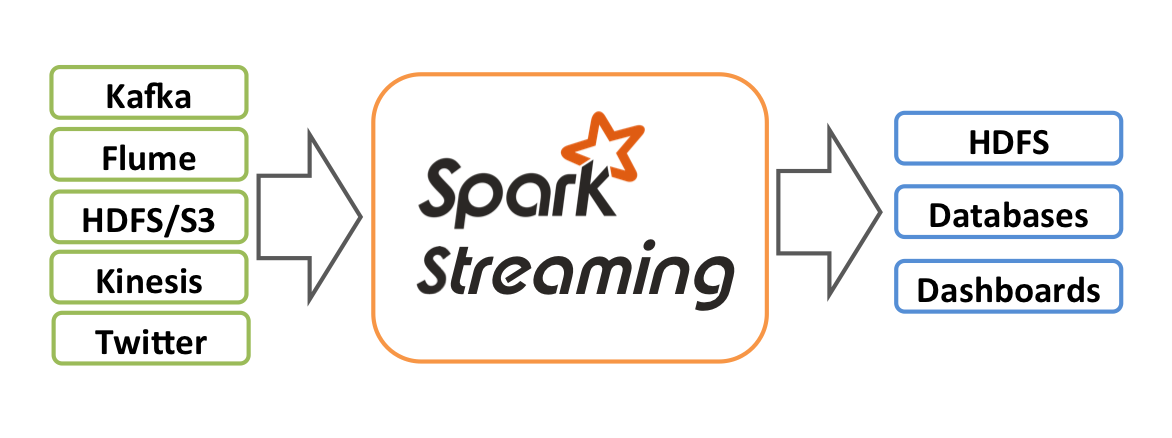
\includegraphics[width=0.8\linewidth]{img/sparkStreaming.png}
	\caption{Funzionalità di Spark Streaming. Immagine tratta da \cite{spark}}
	\label{fig:SparkStreaming}
\end{figure}
\par Una nota di rilevanza fondamentale nello streaming, non supportata da questo modulo è che: esso non riesce a lavorare con il tempo dell'evento, ma solo con l'evento di Spark.

\par Con Spark Streaming, non ci sono restrizioni per utilizzare qualsiasi tipo di sink (``\texttt{foreachRDD}"). %TODO

\par La novità e il maggior supporto sembra sia in Spark Structured Streaming.
\subsubsection{Spark Structured Streaming}
Streaming strutturato, costruito sopra a Spark SQL e dunque con supporto a DataFrame e DataSet. 
Sostanzialmente è possibile riuso totale del codice scritto per interrogazioni statiche su SparkSQL.

Dei benchmarks\footnote{\url{https://blog.knoldus.com/spark-rdd-vs-dataframes}} dimostrano che i DataFrame sono più ottimizzati in termini di elaborazione e forniscono più opzioni per aggregazioni e altre operazioni con una varietà di funzioni disponibili (molte più funzioni sono ora supportate nativamente in Spark 2.4).

Non c'è il concetto di batch di Spark Streaming, assomiglia più a uno stream Real Time.
In ogni caso sotto si procede micro batch, dalla versione 2.3 di spark è stato aggiunto il concetto di \textit{Continuous Processing} che ha ridotto ulteriormente la latenza.

I dati, come mostrato in Figura \ref{fig:StructuredStreaming}, vengono aggiunti a una tabella potenzialemente infinita, composta da una sola colonna 'value' (DataSet<Row>), 
la quale tramite le funzionalità di SparkSQL verrà trasformata nelle colonne opportune.

Per connettersi alle risorse dati bisogna:
\begin{itemize}
	\item Creare una SparkSession
	\item chiamare il metodo readStream() su questa
	\item \texttt{.format()} per specificare il tipo di dato (es. Kafka, Socket, File)
	\item \texttt{.options} per eventuali opzioni come host e porta
\end{itemize}

I dati ottenuti hanno come sink (writeStream): kafka, file, memoria, console
Nota: con il writeStream usando `foreach` e `foreachBatch` è possibile fare quello che voglio, salvare su fonti già presenti, salvare su più fonti.

Ottengo dati in ogni momento.
La modalità in cui si recuperano può essere (dipendentemente dall'interrogazione): 
\begin{itemize}
	\item \textit{Complete}: per ottenere l'output completo di ogni aggiornamento
	\item \textit{Append}: solo righe aggiunte
	\item \textit{Update}: solo righe aggiornate
\end{itemize}

\textbf{Importante}: non viene materializzata l'intera tabella, man mano che vengono interrogati i dati vengono scartati. 

Questo modello è molto differente da altre engine di streaming, molte richiedono all'utente stesso di mantenere aggregazioni sui dati precedenti e sulla loro coerenza.
In questo modello se ne occupa Spark e il tutto rimane trasparente all'utente.

Le modalità di triggering possono essere
\begin{itemize}
	\item default o micro batch mode
	\item fixed
	\item one time
	\item Continuous con un intervallo di checkpoint fissato (sparimentale): continuos processing mode
\end{itemize}

Operazioni supportate:
\begin{itemize}
	\item funzioni di base di SparkSQL 
	\item Window based sliding
	\item \textbf{UDF}\footnote{url{https://jaceklaskowski.gitbooks.io/mastering-spark-sql/spark-sql-udfs.html}}- User defined functions. Si tratta normalissime funzioni scala definite dall'utente, si possono tranquillamente considerare come "black box". Il tutto ha un senso unificato all'utilizzo di case class definite dall'utente rappresentative dei record. Qui nasce il forte senso di structured streaming e assieme al concetto di tempo è qui che secondo
	me c'è il netto distacco con Spark Streaming. MA occhio all'uso di UDF, vedere i piani di esecuzione capire se effettivamente essendo scatole nere ottimizzano l'esecuzione o essa può essere resa meno leggibile ma più performante e comunque eseguibile con i meccanismi offerti da spark / spark sql...inoltre udf ha problemi di seriazzazione, ogni volta deve deserializzare e serializzare le colonne, quando possibile preferire le funzioni builtin che in SparkSQL non sono poche (org.apache.spark.sql.functions). Sono registrabili anche globalmente nella sessione. %TODO meglio
	\item UDAF \footnote{\url{https://jaceklaskowski.gitbooks.io/mastering-spark-sql/spark-sql-UserDefinedAggregateFunction.html}} %TODO
\end{itemize}

Riesce a lavorare con il tempo dell'evento, cosa che non fa Spark Streaming.
Per cui è più adatto al mondo reale, es. IoT.
In caso di ritardi è Spark stesso a preoccuparsi di aggiornare e rimanere con l'event time corretto.
Da Spark 2.1 c'è il \textit{watermarking} che permette all'utente di definire una soglia dei dati in ritardo, e consente, di conseguenza, all'engine di ripulire il vecchio stato.
Occhio alle dimensioni di questo valore, se troppo grande può creare problemi di memoria / performance. Questo è molto importante, delle tipologie di sink non lo supportano in update ma solo in append in modo  che tutto venga scritto alla fine.

Assicura `end-to-end exactly-once semantics` sotto ogni failure.
Oltre al checkpointing per ripristinare la condizione dagli errori, usato anche da Spark Streaming, usa due condizioni:
- La fonti deve essere riproducibili.
- I sink devono supportare operazioni idempotenti per supportare il ritrattamento in caso di guasti.

Con Spark 2.4 lo Structured Streaming ha superato i limiti restringenti che aveva in precedenza sul numero di sink, introducendo un sink `foreachBatch`, questo fornisce la tabella di output risultante
con DataFrame per eseguire operazioni custom.
\begin{figure}
	\centering 
	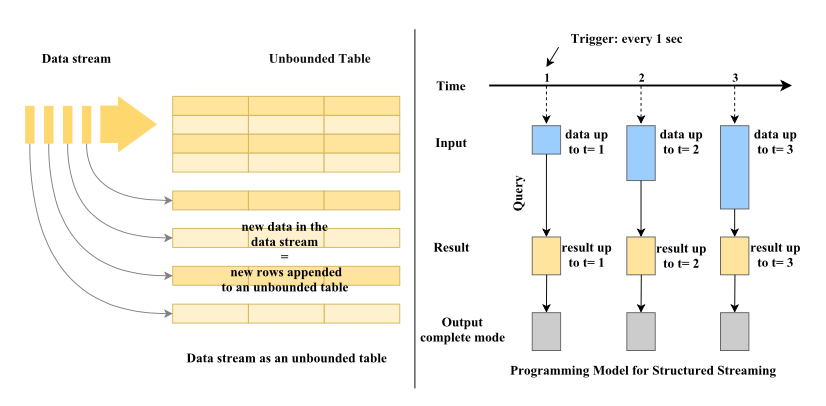
\includegraphics[width=0.8\linewidth]{img/sparkStructuredStreaming.png}
	\caption{Come Spark Structured Streaming mantiene i dati. Immagine tratta da \cite{structuredStreaming}}
	\label{fig:StructuredStreaming}
\end{figure}
\section{Limiti di Spark}
\newpage
\printbibliography
\end{document}
    
%TODO aggiungi cose rimaste
%TODO cita gli esempi e amplia